\frame{
\frametitle{Kela}
\begin{itemize}
\item Ideaalisen kelan toiminta noudattaa yhtälöä
\[
u=L\frac{{\rm d}i}{{\rm d}t}
\]
\item Kela eli käämi eli solenoidi valmistetaan kiertämällä kuparilankaa sydämen ympärille.
\item Sydän voi olla ilmaa, muovia tai magneettista materiaalia.
\item Sydän on yleensä lieriön muotoinen (lieriökäämi) tai toruksen muotoinen (toroidi- eli rengaskäämi).
\item Kelaa, jonka tarkoitus piirissä on virran rajoittaminen, kutsutaan kuristimeksi.  
\item Kelojen käyttöä pyritään yleensä välttämään elektroniikkasuunnittelussa.
\end{itemize}
}

\frame{
\frametitle{Miksi kelojen käyttöä pyritään välttämään}
\begin{itemize}
\item Keloja on kömpelö valmistaa.
\item Kelat vievät paljon tilaa.
\item Kelat aiheuttavat ympärilleen magneettikentän.
\end{itemize}
}

\frame{
\frametitle{Milloin kelojen käyttö on käytännössä pakollista}
\begin{itemize}
\item Hakkuriteholähteet
\item Releet
\item Suurtaajuuslaitteissa kelaa ei voi aina korvata muilla ratkaisuilla.
\end{itemize}
}

\frame{
\frametitle{Käytännön kelan ominaisuudet}
\begin{itemize}
\item Induktanssi toleransseineen
\item Maksimi virrankesto
\item Sarjaresistanssi
\end{itemize}
}

\frame{
\frametitle{Sydänmateriaalin vaikutus}
\begin{itemize}
\item Kelan induktanssi riippuu sydänmateriaalin permeabiliteetista $\mu=\mu_0\mu_{\rm r}$.
\item Diamagneettisilla aineilla (mm. jalometallit) $\mu_{\rm r}$ on aavistuksen verran ykköstä pienempi, paramagneettisilla aineilla kuten ilmalla tai alumiinilla aavistuksen verran ykköstä suurempi.
\item Ferromagneettisilla aineilla $\mu_{\rm r}$ on useita satoja tai jopa yli miljoona.
\end{itemize}
}

\frame{
\frametitle{Pyörrevirtahäviöt}
\begin{itemize}
\item Jos kelan sydän on sähköäjohtavaa materiaalia, sinne indusoituu pyörrevirtoja.
\item Pyörrevirrat aiheuttavat lämpöhäviöitä.
\item Ferriitit ($\rm XOFe_2O_3$) sopivat hyvin sydänmateriaaliksi: niillä on korkea $\mu_{\rm r}$
mutta matala sähkönjohtavuus, jolloin pyörrevirtahäviöt jäävät pieniksi.
\item Yksi tapa vähentää pyörrevirtahäviöitä on käyttää levypakkasydäntä, joka koostuu toisistaan eristetyistä rautalevyistä. Tätä ratkaisua käytetää muun muassa verkkomuuntajissa.
\end{itemize}
}

\frame{
\frametitle{Erilaisia keloja}
\begin{center}
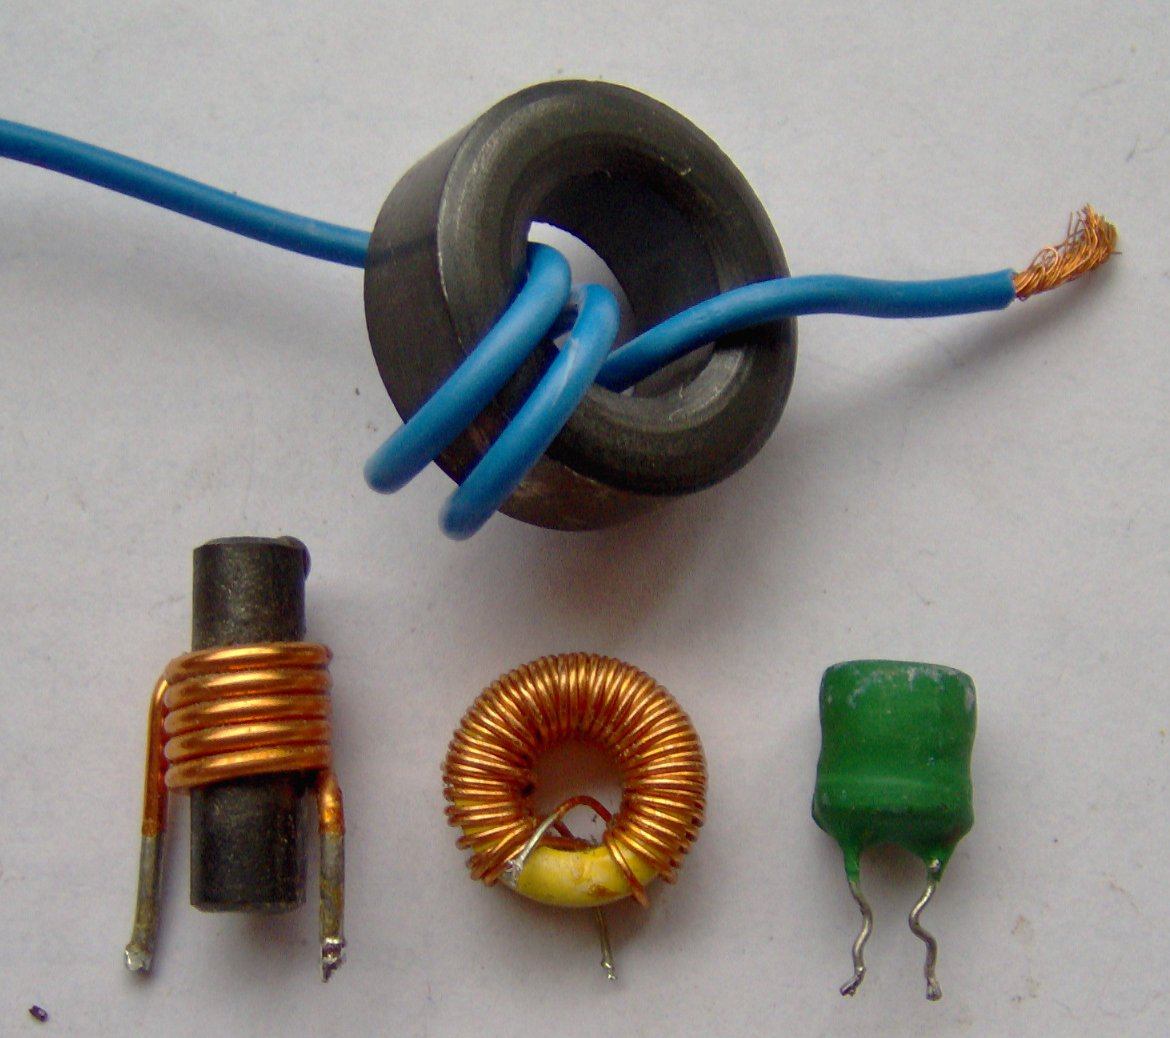
\includegraphics[height=70mm]{kelat_pics/Electronic_component_inductors.jpg}
\end{center}
\tiny \url{http://commons.wikimedia.org/wiki/File:Electronic_component_inductors.jpg} 
}


\frame{
\frametitle{Maxwellin yhtälöt}
Maxwellin yhtälöiden käsittely vaatii yliopistomatematiikkaa. Täällä käydään läpi
vain yhtälöiden merkitys. Maxwellin yhtälöitä on 4:
\begin{itemize}
\item $\nabla \times \vec E=-\frac{{\rm d}B}{{\rm d}t}$ {\bf Faradayn induktiolaki}. Muuttuva magneettikenttä saa aikaan sähkökentän.
\item $\nabla \cdot \vec D=\rho$ {\bf Gaussin laki}. Sähkövaraus $\rho$ saa aikaan sähkökentän.
\item $\nabla \times \vec H=\vec J + \frac{{\rm d}D}{{\rm d}t}$ {\bf Lävistyslaki}. Sähkövirta aikaansaa magneettikentän.
\item $\nabla \cdot \vec B=0$ {\bf Gaussin laki magneettikentille}. Magneettikenttäviivat ovat aina sulkeutuvia eli suljetun pinnan läpi
magneettivuo on nolla.
\end{itemize}
{Maxwellin yhtälöt ovat koko sähkötekniikan perusta.} Niitä ei voi "perustella", ne ovat kokeellisesti
havaittu luonnonlaki, kuten vaikkapa mekaniikasta tuttu $F=ma$.
}


\frame{
\frametitle{Johtimen magneettikenttä}
Maxwellin yhtälöistä voidaan laskea, että suorassa johtimessa kulkeva virta $I$ aikaansaa
magneettikentän, jonka voimakkuus etäisyydellä r johtimesta on $H=\frac{I}{2\pi r}$.
Magneettikenttäviivat kiertävät johdinta.
}

\frame{
\frametitle{Kelan toiminta}
Koska
\begin{itemize}
\item muuttuva magneettikenttä saa aikaan jännitteen johtimeen
\item johtimessa kulkeva virta saa aikaan magneettikentän ja johtimessa kulkeva
muuttuva virta, 
\end{itemize}
niin muuttuva virta johtimessa saa johtimeen aikaan jännitteen joka vastustaa virran muutosta.
Tähän perustuu komponentti nimeltä kela, johon olemme jo tutustuneetkin. Kiertämällä
johdin käämiksi (siis kelaksi) tämä pyrkimys vastustaa virran muutoksia (=induktanssi) kasvaa.
}

\frame{
\frametitle{Muuntajan toiminta}
Kytkemällä kaksi kelaa siten, että toisen magneettikenttä kulkee toisen kelan läpi, syntyy
muuntaja. Tämä voi olla myös ei-toivottu ilmiö. Piirilevyllä lähekkäin kulkevien johtimien
magneettikentät vaikuttavat toisiin johtimiin; tätä ilmiötä kutsutaan {\bf ylikuulumiseksi}.
}



%Seuraavat kaksi kalvoa pöllitty S2010 EMC-kalvoilta ja vähän muokattu

\frame{
\frametitle{Magneettivuo}
\begin{itemize}
\item Magneettivuon tiheys $B$ riippuu magneettikentän voimakkuudesta $H$ ja väliaineen permeabiliteetista $\mu$
\[
B=\mu H
\]
\item Vuontiheyden yksikkö on tesla (T). Puhekielessä magneettikentän voimakkuus ja magneettivuon tiheys menevät usein sekaisin (esim. mitataan vuontiheyttä ja puhutaan kentänvoimakkuudesta).
\item Pinta-alan $A$ läpi kulkeva magneettivuo $\phi$ on
\[
\phi = \int_A \vec{B}\cdot {\rm d} \vec{A}
\]
\end{itemize}
}


\frame{
\frametitle{Sähkömagneettinen induktio}
\begin{itemize}
\item Faradayn lain mukaan muuttuva magneettivuo $\phi$ indusoi käämiin jännitteen, jonka suuruus on
\[
e=-\frac{{\rm d}\phi }{{\rm d}t}
\]
\item Koska vuontiheys on sitä suurempi mitä suurempi on permeabiliteetti ja vuontiheyden muutosnopeus vaikuttaa induktiojännitteeseen, on kelan induktanssi suoraan verrannollinen sydämen
suhteelliseen permeabiliteettiin $\mu_{\rm r}$.
\end{itemize}
}


\frame{
\frametitle{Hystereesi}
\begin{itemize}
\item Ferromagneettisilla aineilla $\mu_{\rm r}$ on hyvin suuri, mutta myös voimakkaasti riippuvainen magneettikentän voimakkuudesta!
\item Suurilla kentänvoimakkuuksilla materiaali {\em kyllästyy} ja $\mu_{\rm r}$ pienenee mitä suuremmaksi magneettikentän voimakkuus kasvaa.
\end{itemize}
}

\frame{
\frametitle{Hystereesi}
\begin{center}
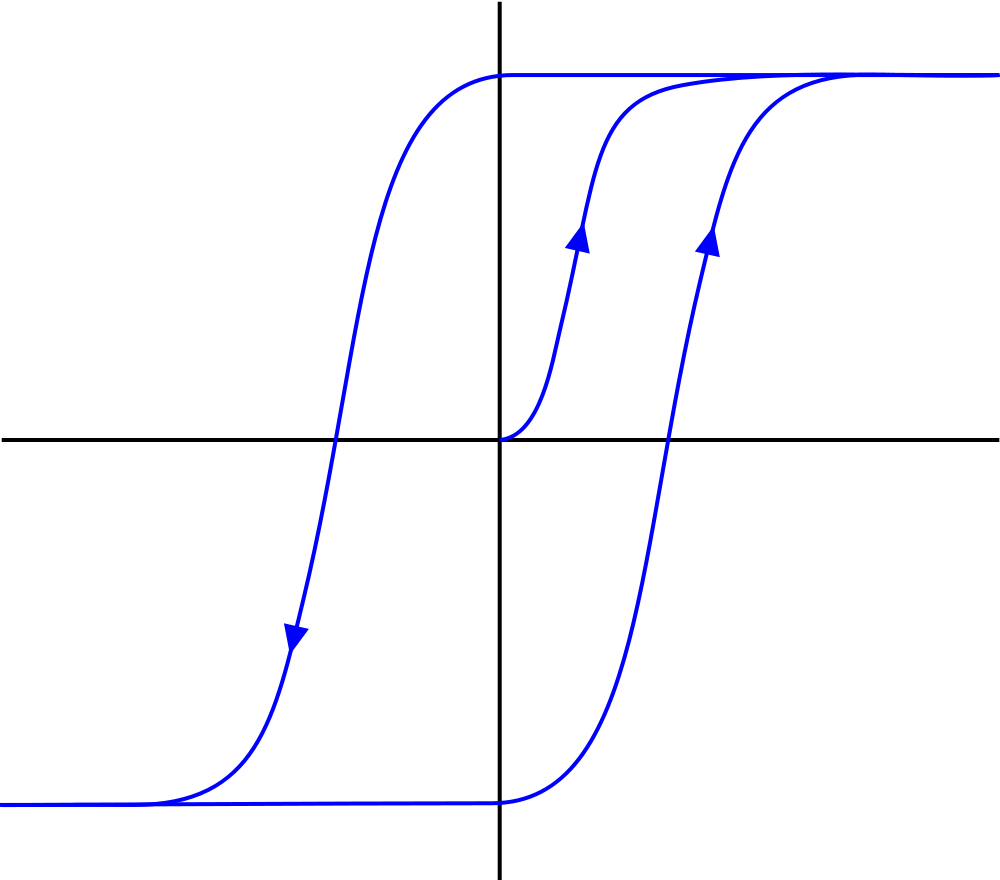
\includegraphics[height=70mm]{kelat_pics/1000px-Hysteresiscurve.png}
\end{center}
\tiny \url{http://commons.wikimedia.org/wiki/File:Hysteresiscurve.svg} 

}
